\subsection{Tellbarhet}
\begin{frame}{Hva er størst av $|\mathbb{N}|$ og $|\mathbb{Z}|$?}
    \begin{columns}
    \begin{column}{0.35\textwidth}
        $\mathbb{N} = \{0, 1, 2, 3, 4, ...\}$\\
        $\mathbb{Z} = \{..., -2, -1, 0, 1, 2, ...\}$\\[5mm]
        \pause
        Vi definerer en bijeksjon:\\ 
        $f : \mathbb{N} \rightarrow \mathbb{Z}$
        $f(n) :=
        \begin{cases}
            \frac{n}{2}, n \text{ mod } 2 = 0\\
            -\frac{n+1}{2}, \text{otherwise}\\
        \end{cases}$\\[5mm]
        \pause
        Konklusjon: $|\mathbb{N}|$ = $|\mathbb{Z}|$ = $\aleph_0$. 
    \end{column}
    \begin{column}{0.6\textwidth}
        \begin{figure}
            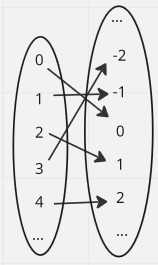
\includegraphics[scale=0.75]{images/n eq eq z.png}
        \end{figure}
    \end{column}
    \end{columns}    
\end{frame}

\begin{frame}{Hva er størst av $|\mathbb{N}|$ og $|\mathbb{Q}|$?}
        $\mathbb{N} = \{0, 1, 2, 3, 4, ...\}$\\
        $\mathbb{Q} = \{a / b | a, b \in \mathbb{Z}\}$\\[2mm]
        \pause
        Vi definerer en bijeksjon $g : \mathbb{N} \rightarrow \mathbb{Q}$:\\
        $f(0) := 1$\\
        $f(n) := \frac{1}{2\lfloor f(n-1) \rfloor - f(n-1)+1}$\\
        $g(0) := 0$\\
        $g(2n) := f(n)$\\
        $g(2n-1) := -f(n)$\\
        Konklusjon: $|\mathbb{N}|$ = $|\mathbb{Q}|$ = $\aleph_0$.\\[2mm]\pause
        Derimot er $|\mathbb{R}| > |\mathbb{N}|$, og vi skriver at $|\mathbb{R}| = \aleph_1$.\\ 
        For en enkel forklaring med et eksempel, se Veritasiums video om Hilberts Hotell: \url{https://www.youtube.com/watch?v=OxGsU8oIWjY}
\end{frame}